%\chapter*{Неделя 11}
\protect\thispagestyle{fancy}
\section{}
На рисунке изображён спектр узкополосного сигнала. Пусть полоса $B=f_2-f_1=100$ KHz и сигнал дискретизуется с частотой $f_d = 2B$, $f_3 = (f_1 + f_2)/2$.

Изобразить спектр дискретизованного сигнала в полосе $[-f_2; f_2]$ для каждого из трёх случаев:

\begin{figure}[h]
	\centering
	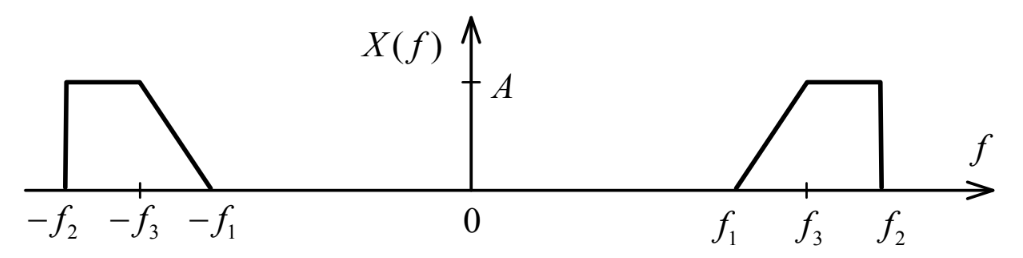
\includegraphics[width=0.8\linewidth]{pics/spring/11/11-1-0.png}
	%\caption{.}
	\label{fig:11-1-0}
\end{figure}


\begin{center}
	1) $\dfrac{f_2}{B} = 3$,\quad 2) $\dfrac{f_2}{B} = 4$,\quad 3) $\dfrac{f_2}{B}=4.5$.
\end{center}
Обосновать результаты.

\begin{figure}[h]
	\centering
	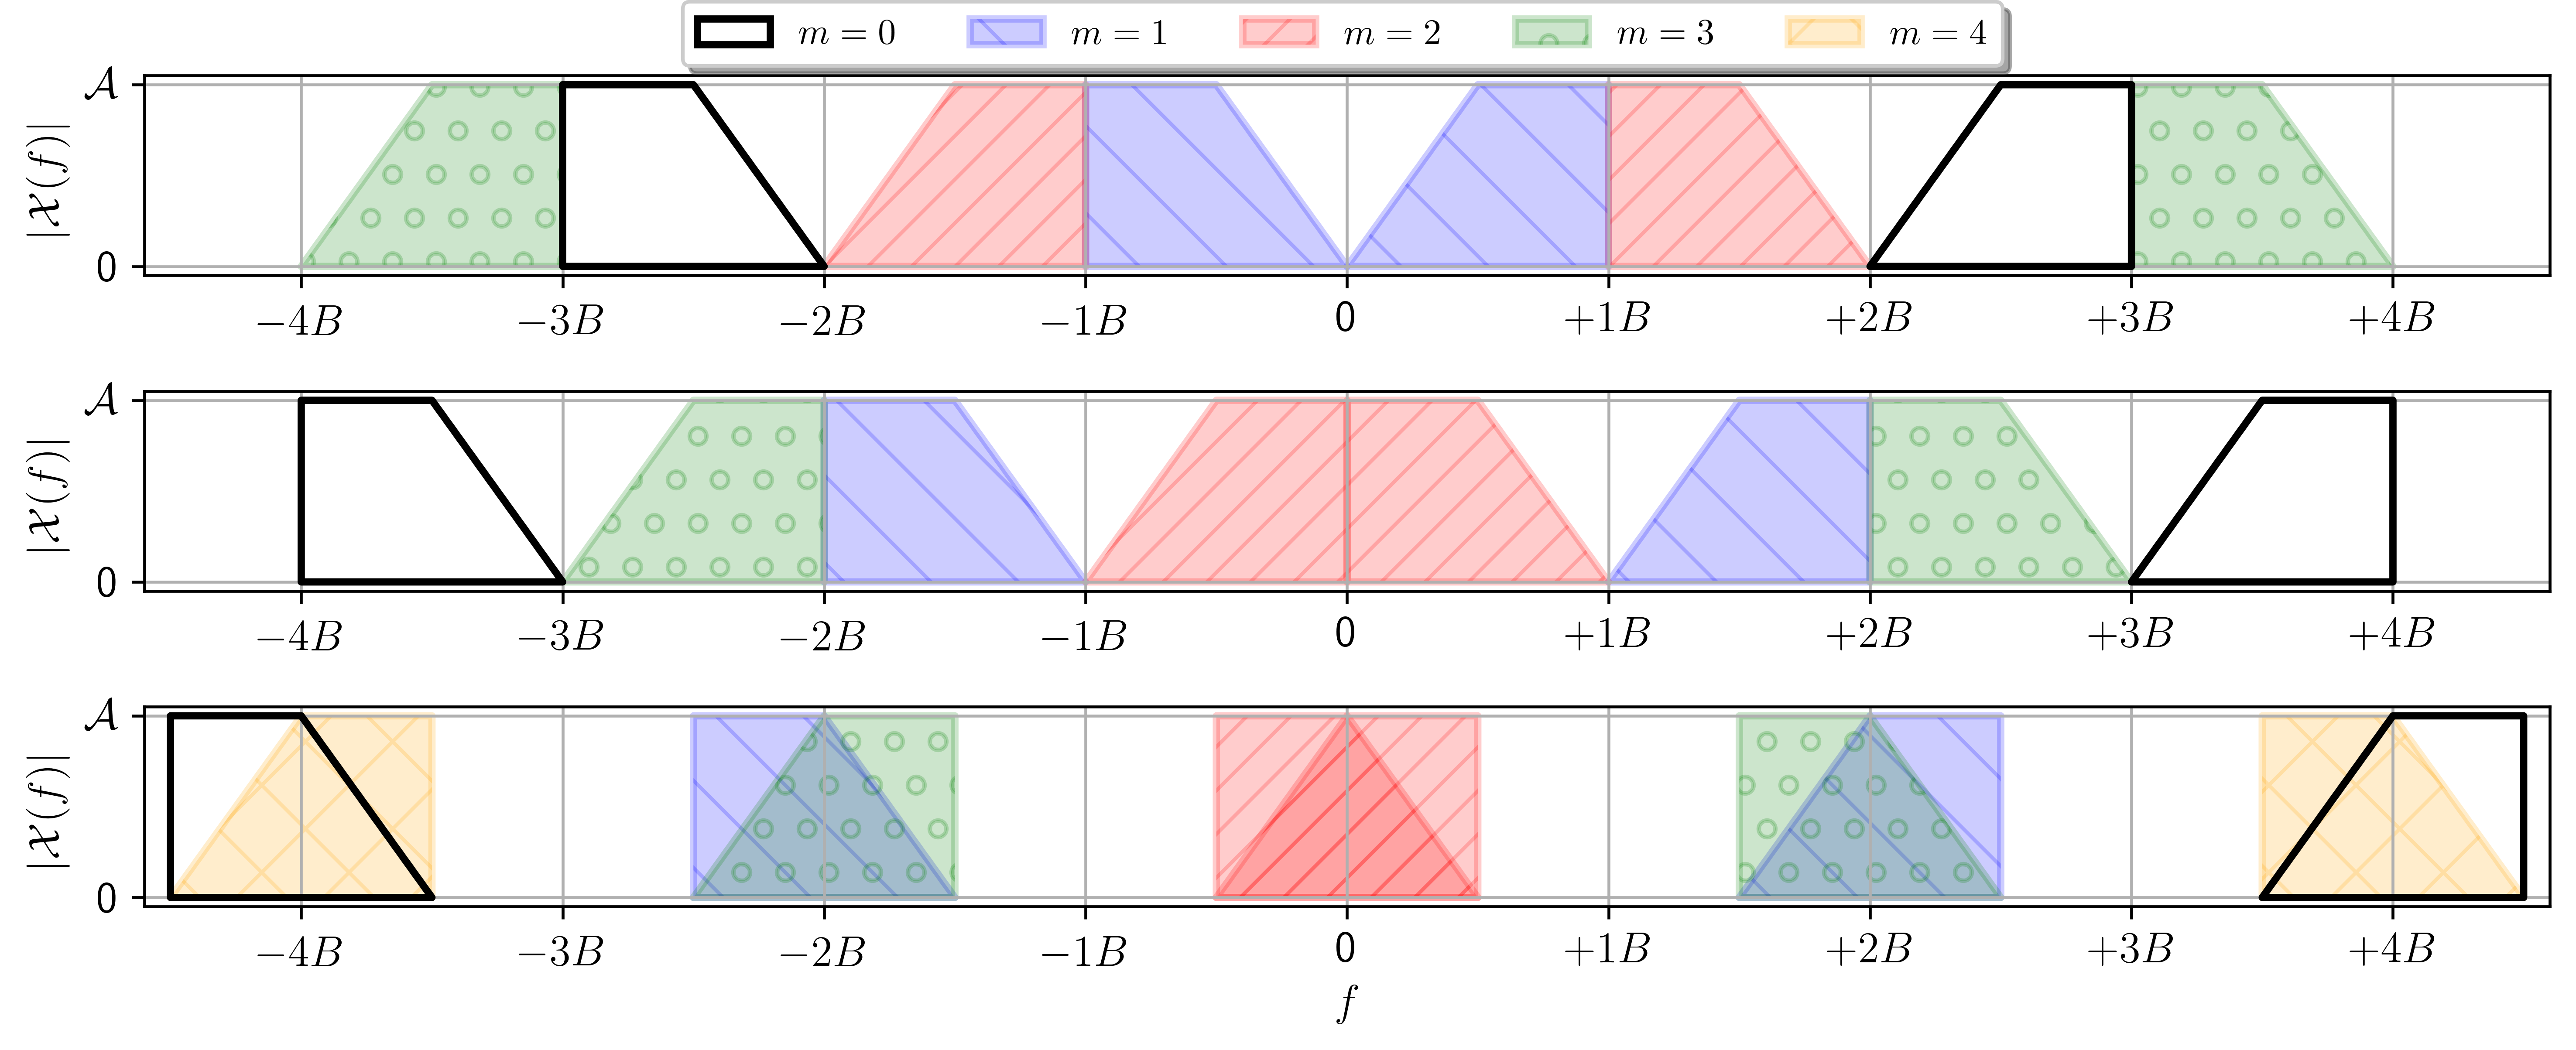
\includegraphics[width=\linewidth]{pics/spring/11/11-1-1.png}
	%\caption{.}
	\label{fig:11-1-1}
\end{figure}

Выше представлены графики дискретизованного сигнала для трёх случаев соответственно. Разными цветами обозначены изображения спектра с различными порядками субдискретизации $m$.

В первых двух случаях имеет место целочисленное деление полос ($f_2/B = \{3, 4\} \in \mathbb{N}$) с минимальной частотой дискретизации $f_d = 2(f_2 - f_1) = 2B$. Поэтому мы наблюдаем плотную упаковку спектров без какого-либо эффекта наложения. Разница между случаями $1$ и $2$ заключается лишь в том, что в первую зону Найквиста спектр отображается с разной кратностью переноса ($m$) с возможной инверсией, наличие которой зависит от расположения исходного сигнала.


В третьем случае реализуется случай нецелочисленных полос ($f_2/B = 4.5 \notin \mathbb{N}$). Минимальная частота дискретизации, при которой отсутствует наложение спектров, находится из условия:

\begin{equation*}
\dfrac{2f_2}{m+1} \leq f_d \leq \dfrac{2f_1}{m} \quad \Leftrightarrow \quad \dfrac{9B}{m+1} \leq f_d \leq \dfrac{7B}{m}.
\end{equation*}
Откуда можно легко получить, что $f_d/B \in \left[9/4; 7/3\right] \cup \left[3; 3.5\right] \cup [4.5; 7]$, то есть ${f_d}_{\min} = 2.25B$. 
В условии задачи предлагается использовать $f_d = 2B$, что меньше минимально возможной <<хорошей>> частоты. Поэтому мы наблюдаем наложение спектров при субдискретизации.


\section{}
На рис.~а) показано устройство предварительной обработки данных приёмника многоканальной системы связи.

\begin{figure}[h]
	\centering
	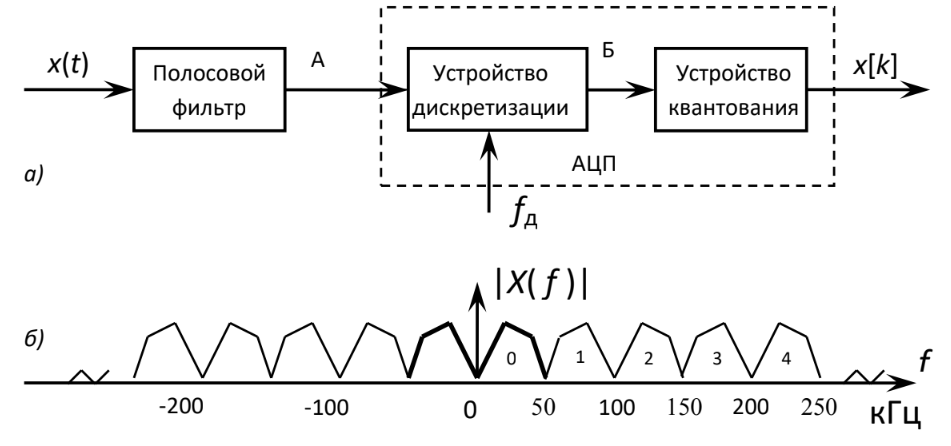
\includegraphics[width=0.8\linewidth]{pics/spring/11/11-2-0.png}
	%\caption{.}
	\label{fig:11-2-0}
\end{figure}


Спектр принимаемого сигнала показан на рис.~б) с указанием номеров каналов. Для выделения сигнала в нужном канале служит полосовой фильтр. Будем считать его идеальным.

\begin{itemize}
	\item Найти минимальную частоту дискретизации ${f_d}_{\min}$ для канала $4$ при условии, что реализуется субдискретизация полосового сигнала.
	\item Изобразить модуль спектра дискретного сигнала (точка Б) в полосе $[-f_d/2, f_d/2]$.
\end{itemize}

Следуя обозначениям первой задачи, для канала $4$ имеем: $f_1 = 200$ kHz, $f_2 = 250$ kHz, $B = f_2 - f_1 = 50$ kHz. Легко видеть, что как $f_1$, так и $f_2$ оказываются кратны $B$, что позволяет выбирать частоту дискретизации только лишь по критерию Найквиста: $f_d \geq 2B = 100$ kHz, ${f_d}_{\min} = 100$ kHz.

Аналогичный результат можно получить из более общего рассмотрения, включающего случай нецелочисленных полос. Пересечения изображений спектра будут отсутствовать, если:

\begin{equation*}
\begin{cases}
f_d/B \geq 2\\
\dfrac{2f_2}{m+1} \leq f_d \leq \dfrac{2f_1}{m},\; m \in \mathbb{N}
\end{cases} \Rightarrow \;
f_d/B \in \{2\} 
\cup \left[\dfrac{10}{4}; \dfrac{8}{3}\right] 
\cup \left[\dfrac{10}{3}; \dfrac{8}{2}\right]  
\cup \left[\dfrac{10}{2}; \dfrac{8}{1}\right]  \Rightarrow \;
{f_d}_{\min} = 2B = 100 \text{ kHz.}
\end{equation*}

График спектра в точке Б представлен ниже. Можно видеть, что в первую зону Найквиста попадает изображение спектра исходного сигнала без инверсии.
\begin{figure}[h]
	\centering
	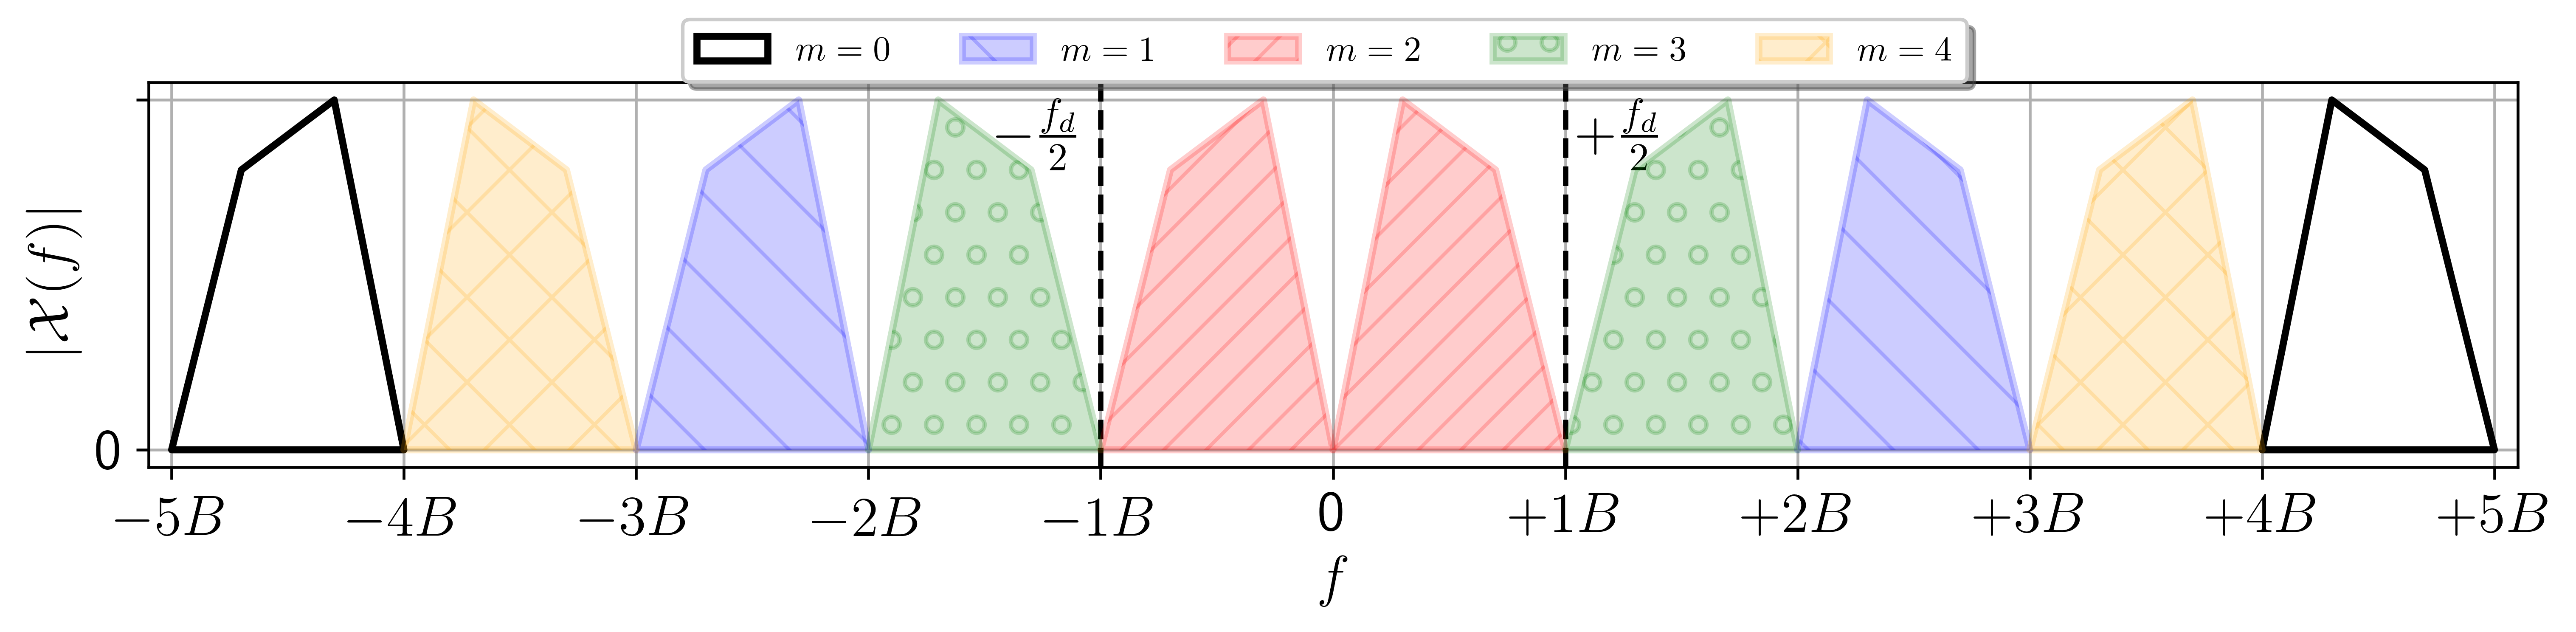
\includegraphics[width=\linewidth]{pics/spring/11/11-2-1.png}
	%\caption{.}
	\label{fig:11-1-2}
\end{figure}

\section{}
Показать, что спектр действительного цифрового сигнала $x[k]$ можно инвертировать

\begin{equation*}
\Capit{Y}(\nu) = \Capit{X}(\nu-0.5)
\end{equation*}

путём изменения знака каждого второго отсчёта сигнала $x[k]$:
\begin{equation*}
y[k] = (-1)^k x[k],\; k=0,1,2,\ldots.
\end{equation*}

\begin{equation*}
\Capit{X}(\nu) = \sum_{\{k\}} x[k]\exp\left(-j 2\pi \nu k\right), \quad \Capit{Y}(\nu) = \sum_{\{k\}} y[k]\exp\left(-j 2\pi \nu k\right).
\end{equation*}

\begin{align*}
\Capit{X}(\nu-0.5) &= \sum_{\{k\}} x[k]\exp\left(-j 2\pi (\nu - 0.5) k\right) = \sum_{\{k\}} x[k]\exp\left(-j 2\pi \nu k\right)\exp\left(+j \pi k\right) = \\
&=\sum_{\{k\}}(-1)^k  x[k] \exp\left(-j 2\pi \nu k\right) = \sum_{\{k\}}y[k] \exp\left(-j 2\pi \nu k\right) = \Capit{Y}(\nu).
\end{align*}

